\documentclass[10pt, oneside]{article}

\input ./combined_macros.sty

\addbibresource{Twist.bib}

\usepackage{pdflscape}
\usetikzlibrary{shapes.geometric, arrows, positioning}

\tikzstyle{s16} = [rectangle, rounded corners, minimum width=1.8cm, minimum height=1cm,text centered, draw=black,fill=red!30]
\tikzstyle{s16chiral} = [s16, dashed]
\tikzstyle{s8} = [rectangle, rounded corners, minimum width=1.8cm, minimum height=1cm,text centered, draw=black,fill=orange!30]
\tikzstyle{s4} = [rectangle, rounded corners, minimum width=1.8cm, minimum height=1cm,text centered, draw=black,fill=yellow!30]
\tikzstyle{s2chiral} = [rectangle, dashed, rounded corners, minimum width=1.8cm, minimum height=1cm,text centered, draw=black,fill=green!30]
\tikzstyle{dimension} = [circle, text centered, text width=0.7cm, minimum height=0.7cm, draw=black]
\tikzstyle{arrow} = [thick,->,>=stealth]

\title{Twists of supersymmetric gauge theories}
\author{Chris Elliott\and Pavel Safronov \and Brian Williams}

\date{\today}

\begin{document}

\maketitle

\section*{Introduction}

\section{The BV-BRST Formalism}

Throughout the paper we will mostly work with a $\ZZ\times\ZZ/2$-grading. \emph{Degree} will refer to the first (cohomological) grading and \emph{odd} or \emph{even} to the second (fermionic) grading.

\subsection{Classical BV Theories}

\begin{dfn}
A {\bf free BV theory} on a manifold $M$ is the data:
\begin{itemize}
\item a finite rank $\ZZ\times\ZZ/2$-graded vector bundle $E \to M$ equipped with an even differential operator of cohomological degree $+1$
\[
Q \colon \cE \to \cE [1] 
\]
such that $(1)$: $Q^2 = 0$ and $(2)$: the pair $(\cE , Q)$ is an elliptic complex;
\item a map of bundles
\[
\omega\colon E \otimes E \to {\rm Dens}_M [-1]
\]
that is
\begin{enumerate}
\item[$(1)$] fiberwise nondegenerate,
\item[$(2)$] graded skew symmetric, and
\item[$(3)$] satisfies $\int_M \omega\<e_0, Q e_1\> = (-1)^{|e_0|} \int_M \omega(Q e_0, e_1)$ where $e_i$ are compactly supported sections of $E$ .
\end{enumerate}
\end{itemize}
\end{dfn}

\brian{recall dfn of $\oloc$ of a gr vb.} \chris{before the definition below we should probably define the antibracket $\{,\}$ (in terms of the shifted symplectic structure).}

\begin{dfn}
A {\bf classical BV field theory} (or simply, classical field theory) is a free BV theory $(E, Q, \omega)$ equipped with an even functional
\[
I \in \oloc^+(E)
\]
of cohomological degree zero satisfying the classical master equation 
\[
Q I + \frac{1}{2} \{I,I\} = 0 .
\]
\end{dfn}

Given a classical field theory $(E, Q, \omega, I)$ we denote by
\[S = \frac{1}{2} \int_M \omega(e, Q e) + I\in \oloc(E)\]
the BV action of the theory.

\begin{remark}
We will also consider $\ZZ/2$-graded classical field theories which are defined as before, but where $E$ has only a single $\ZZ/2$-grading and, correspondigly, $Q$ is simply an odd operator.
\end{remark}

A local functional induces an endomorphism $\{I,-\}$ on the space of all local functionals $\oloc(E)$. 
It also induces an endomorphism on the larger space of {\em all} functionals $\cO(\cE)$, see Definition \ref{dfn: fnl} in the appendix. 
The classical master equation implies that the operator $Q + \{I,-\}$ squares to zero on $\cO(\cE)$, and hence every classical field theory defines a cochain complex
\begin{equation}\label{bvcplx}
\left(\cO(\cE), Q + \{I,-\}\right) .
\end{equation}
In fact, this has the structure of a differentiable pro-cochain complex, see Definition \ref{dfn: pro}. 
We will refer to this as the {\bf classical BV complex} of the theory. 

\begin{dfn}
A {\bf morphism} of classical field theories (defined on the same manifold $M$) $F\colon (E, Q, \omega, I) \to (E', Q', \omega', I')$ is a linear map of vector bundles
\[
F\colon E \to E'
\]
that intertwines the differentials $Q, Q'$, the pairings $\omega, \omega'$, and the interactions $I,I'$. 
\end{dfn}

Note that a map of classical field theories induces a map of BV complexes, that is, a map of pro-cochain complexes:
\[
F^*\colon \left(\cO (\cE)[-1], Q + \{I,-\} \right) \to \left(\cO (\cE')[-1], Q' + \{I',-\} \right) .
\]
This allows us to make the following definition of an equivalence between classical theories. 

\begin{dfn} \label{equivalence_def}
A morphism of classical field theories $F\colon (E, Q, \omega, I) \to (E', Q', \omega', I')$ is an {\bf equivalence} if it induces a quasi-isomorphism of differentiable pro-cochain complexes
\[
F^* \colon  \left(\cO(\cE')[-1], Q' + \{I',-\} \right) \xto{\simeq} \left(\cO(\cE)[-1], Q + \{I,-\} \right) .
\]
\end{dfn}

For a short background on homological algebra with differentiable pro-cochain complexes, including the notion of quasi-isomorphism, we refer to Appendix \ref{appx: top}.
For a more thorough introduction, and for which our conventions are based on, we refer to \cite{CG1}. 

\begin{dfn} \label{infinitesimal_action_def}
Let $(E, Q,\omega, I)$ be a classical field theory 
A {\bf strict action} of a super Lie algebra $\fg$ on $(E, Q,\omega, I)$ is a map of super dg Lie algebras (in differentiable pro-cochain complexes)
\[
\rho\colon \fg \to \left(\oloc(E)[-1] , \{-,-\}_\omega, Q + \{I,-\}_\omega\right) .
\]
More generally, an $L_\infty$ {\bf action} is an $\infty$-morphism of super dg Lie algebras
\[
\rho\colon \fg \rightsquigarrow \left(\oloc(E)[-1] , \{-,-\}_\omega, Q + \{I,-\}_\omega\right) .
\]
\brian{maybe point to appendix where we can fix conventions for $\infty$-maps} \chris{Can we also give the definition here of an equivariant classical field theory in terms of the Maurer-Cartan / equivariant classical master equation?}
\end{dfn}

We denote components of an $\infty$-morphism by $\rho_2, \rho_3, \dots$, so that $\rho_2$ is a morphism of (super) chain complexes. \chris{below we define it in terms of an interaction with components $I^{(1)}, I^{(2)}$ etc, so we should give that point of view here as well.}

\subsection{The Classical Factorization Algebra}

\pavel{explain how to obtain a factorization algebra from a classical field theory.}

Let $(E, Q, \omega, I)$ be a classical BV theory. 
%and suppose $\psi_0 \in \sE$ is a fixed solution to the equations of motion. 
We recall the formalism of \cite{CG1,CG2} which extracts a factorization algebra on spacetime.

\begin{dfn}
Let $(E, Q, \omega, I)$ be a classical field theory on $M$.
The {\bf classical factorization algebra of observables} $\Obs$ assigns to an open set $U \subset M$ the commutative dg algebra (in differentiable pro-cochain complexes)
\[
\Obs(U) = \left(\cO(\cE(U)) , Q + \{I,-\}\right) .
\]
\end{dfn}

Notice that the BV complex we defined in the previous section, Equation (\ref{bvplx}), is the global sections of the factorization algebra along $M$.
The BV complex can be thought of as the complex of functions on the derived critical locus of the action functional.
It makes sense to restrict fields to any open set $U \subset M$. 
Thus, likewise, the value of the factorization algebra on an open set $U \subset M$ can be interpreted as functions on the critical locus of the action functional where we restrict the theory to $U$. 

The fact that the assignment $U \mapsto \Obs(U)$ defines a factorization algebra can be found in Proposition ?? of \cite{CG2}. 

\subsection{From BRST to BV}

\begin{dfn}
A {\bf classical BRST theory} on a manifold $M$ consists of the following data:
\begin{itemize}
\item a $\ZZ$-graded vector bundle $F$ together with the structure of a local $L_\infty$ algebra on the shift $F[-1]$;
\item a differential operator
\[
Q_{BRST} : \cF \to \cF^!  ;
\]
\item a local functional $I_{BRST} \in \oloc^+(\cF)$ of polynomial degree $\geq 3$.
\end{itemize}
Together, this data must satisfy the master equation
\[
[\d_{CE}, Q_{BRST}] + \d_{CE} I_{BRST} = 0 .
\]
where $\d_{CE}$ is the Chevalley-Eilenberg differential defined by the $L_\infty$ structure on $F[-1]$. 
\brian{even separately, I suppose?}
\end{dfn}

We can unwrap this definition as follows. 
One can think of the space of field $\cF$ as a (linear) graded manifold.
In doing so, the $L_\infty$ structure on $\cF[-1]$ determines a vector field $X$ of cohomological degree $+1$ on this graded manifold. 
The operator $Q$ determines a one-form on $\cF$, and the master equation says that this one-form vanish along the vector field $X$. 
Similarly, the condition $\d_{CE} I = 0$ means the function $I$ on $\cF$ vanish along $X$. 

From a classical BRST theory $(\cF, Q_{BRST}, I_{BRST})$, one can construct a classical BV theory as follows. 
Let $\{\ell_k\}$ be the $L_\infty$ structure maps underlying the local Lie algebra $F[-1]$. 

First, we define the free BV theory. 
This will only use the linear operation on the $L_\infty$ algebra $\cF$, and the operator $Q_{BRST}$. 
The underlying bundle of the BV theory is
\[
E = F \oplus F^! [-1] = F \oplus F^* \otimes {\rm Dens}_M .
\]
The differential of the free BV theory is
\[
Q = \ell_1 + Q_{BRST} .
\]
The BV pairing $\omega_{F}$ is defined by the composition
\[
E \otimes E = (F \oplus F^![-1]) \otimes (F \oplus F^![-1]) \to F \otimes F^! [-1] \oplus F^![-1] \otimes F \to {\rm Dens}_M [-1] .
\]
The first arrow is the obvious projection. 
The second arrow is given by the evaluation pairing between $F$ and $F^*$. 
It's immediate to check that the data $(\cE, Q, \omega)$ defines a free BV theory. 

The interacting theory is constructed as follows.
First, note that for $k \geq 2$ the $L_\infty$ structure maps $\{\ell_k\}_{k \geq 2}$ on $\cF$ pull back to multilinear maps on $\cE$ via the obvious projection $p : \cE = \cF \oplus \cF^![-1] \to \cF$. 
These structure maps assemble into a local functional $I_F \in \oloc^+(\cE)$ defined by
\[
I_{F} (e) = \sum_{k \geq 2} \int_M \frac{1}{(k+1)!} \omega_F(e, (p^*\ell_k) (e, \ldots, e)) . 
\] 
Likewise, the BRST action $I_{BRST}$ pulls back to $\cE$, and we define the BV interaction as the sum
\[
I_{BV} = I_{F} + p^* I_{BRST} \in \oloc^+(\cE) .
\]

\begin{lemma}
Given a classical BRST theory $(F, Q_{BRST}, I_{BRST})$, the data $(E, Q, \omega, I) = (F \oplus F^![-1] , \ell_1 + Q_{BRST} , \omega_F, I_{BV})$ defines a classical BV theory.
That is, the BV classical master equation
\[
Q I + \frac{1}{2} \{I, I\} = 0 \iff (Q + \ell_1) (I_F + p^*I_{BRST}) + \frac{1}{2} \{I_F + p^*I_{BRST}, I_F + p^*I_{BRST}\} = 0
\]
holds.
We refer to this classical BV theory as the {\bf $(-1)$-shifted cotangent bundle} of $\cF$ and by abuse of notation we often denote it simply by $\cE = T^*[-1] \cF$.
\end{lemma}

\begin{proof}
\brian{shouldn't be hard...}
\end{proof}

%\begin{dfn}
%A {\bf classical BRST theory} is a finite rank $\ZZ \times \ZZ / 2$-graded vector bundle $F \to M$ equipped with an even differential operator of cohomological degree $+1$
%\[
%Q : \cF \to \cF[1]
%\]
%such that $Q

\subsection{Examples of BV-BRST Theories}

\brian{should we make these definitions, recollections, or just conventions?}

If $M$ is a smooth manifold, its {\em de Rham stack}, as a dg ringed space, is 
\[
M_{\rm dR} = \left(M , (\Omega^\bu_M, \d_{\rm dR})\right) .
\] 

If $X$ is a complex manifold, there are two naturally associated dg ringed spaces that will be important for us. 
The first is the $\dbar$-{\em stack}, defined by
\[
X_{\dbar} = \left(M , (\Omega^{0,\bu}_X, \dbar) \right) .
\]
The next is the {\em Dolbeault stack}, defined by
\[
X_{\rm Dol} = \left(M, (\Omega^{\bu,\bu}_X, \dbar)\right) .
\] 
Note that as sheaves of dg modules, there is a quasi-isomorphism $(\Omega^{p,*}_M, \dbar) = \Omega^{p, hol}_M$.
Thus, one can think of the underlying ring of the Dolbeault stack as functions on the shifted holomorphic tangent bundle $T^{1,0} [1] M$ of $M$. 

\subsubsection{Mixed holomorphic/topological BF theory}

\begin{dfn}
Let $X,Y$ be complex manifolds and $M$ a smooth manifold.
Let $\fg$ be an $L_\infty$ algebra which is finite dimensional in each cohomological degree. 
The {\bf mixed holomorphic-Dolbeault-topological BRST theory} \brian{blah, terrible name} \chris{I don't really understand why this thing needs a name, since it's only a theory in a trivial way, with zero action.  Why not just call this thing $\cF$, call its shifted cotangent something like ``generalized BF theory'', then if $\fg$ has a pairing call the theory built out of $\cF$ with its AKSZ structure something like ``generalized Chern-Simons theory'' (I'm brainstorming other names too: e.g. ``Hodge-Chern-Simons theory'')?  Or do you want to reserve the name Chern-Simons for the case where $\fg$ is a Lie algebra, not an $L_\infty$ algebra?} on $X \times Y \times M$ is the local $L_\infty$ algebra defined by
\[
\cF[-1] = \Omega^{0,\bu}_X \Hat{\otimes} \Omega^{\bu,\bu}_Y \Hat{\otimes} \Omega^\bu_M \otimes \fg .
\] 
The $L_\infty$ structure is the one induced from $\fg$ together with the dg commutative product on differential forms. 
This is a classical BRST theory by choosing $Q_{BRST} = 0$ and $I_{BRST} = 0$. 
In other words, $\cF$ is defined by the mapping stack
\[
{\rm Map} (X_{\dbar} \times Y_{\rm Dol} \times M_{\rm dR}, B \fg) .
\]

The {\bf mixed holomorphic-Dolbeault-topological BF theory} is the BV theory given by the $(-1)$-shifted cotangent bundle to $\cF$.
\end{dfn}

Unpacking the definition \brian{unpack and write out action explicitly?} 

\subsubsection{Mixed holomorphic/topological Chern-Simons theory}

The next class of examples of classical BV theories we give are generalizations of Chern-Simons theory. 
Unlike the examples of mixed BF theory above, these BV theories do not arise, in general, as shifted cotangent bundles. 

Fix a Calabi-Yau manifold $X$ of {\em complex} dimension $n$, a smooth manifold of {\em real} dimension $m$, and let $\fg$ be a $\ZZ/2$-graded Lie algebra with a non-degenerate graded symmetric pairing of parity opposite to $n+m$. 
In particular, if $n+m$ is odd, we can take an ordinary complex semi-simple Lie algebra $\fg$ with its Killing form. 
When $n+m$ is even, we must work with a graded Lie algebra with an odd pairing.
In any case, we denote the pairing on $\fg$ by $\<-,-\>$. 

\begin{dfn}
Let $X, M$, and $\fg$ be as above.
{\bf Mixed Chern-Simons theory} on $X \times M$ with values in $\fg$ is the $\ZZ/2$-graded classical field theory $(E_\mCS, Q_\mCS, \omega_\mCS, I_\mCS)$, where the space of fields is given by
\[
\cE_\mCS = \Omega^{0,\bullet}(X) \Hat{\otimes} \Omega^\bu(M) \otimes \fg [1] .
\]
The linear part of the BV differential is
\[
Q_{\mCS} = \dbar \otimes 1 \otimes 1 + 1 \otimes \otimes 1 \otimes \d_{\dR}
\]
where $\dbar$ is the Dolbeault differential on $X$, and $\d_{\dR}$ is the de Rham differential on $M$.
The pairing $\omega_\hCS$ is
\[
\omega_{\hCS} (\alpha,\beta) = \<\alpha \wedge \beta\> \wedge \Omega_X ,
\]
where $\Omega_X$ is the Calabi-Yau structure on $X$.
Finally, the interaction $I_\hCS$ is
\[
I_{\hCS}(\alpha) = \frac 16 \<\alpha \wedge [\alpha, \alpha]\> \wedge \Omega_X .
\]
As a mapping stack, mixed Chern-Simons is given by
\[
{\rm Map} (X_{\dbar} \times M_{\dR} , B \fg) .
\]

\end{dfn}

By convention, when $X$ is the trivial complex manifold we take $\Omega_X = 1$. 

\begin{eg}
The most basic  example is to take $X$ trivial and $\dim_{\RR} (M) = 3$.
Then we obtain ordinary Chern-Simons theory on $M$. 
Of course, this theory admits an obvious lift to a $\ZZ$-graded BV theory. 
\end{eg}

\begin{eg} 
Now, take $M$ to be trivial and let $X$ be a Calabi-Yau $2$-fold, like $\CC^2$.
Since $n + m = 2$ is even, we must take a graded Lie algebra with odd pairing. 
First, let $\fh$ be an ordinary Lie algebra equipped with an invariant non-degenerate symmetric pairing $\<-,-\>_\fh$. 
Define the $\ZZ/2$-graded Lie algebra
\[
\fg = \fh[\epsilon_1,\epsilon_2, \epsilon_3] 
\]
where $\epsilon_i$ are odd formal variables. 

There is an odd pairing on $\fg$ defined using the pairing on $\fh$ and the Berezin integral along the odd coordinates:
\[
\<X , Y\> = \int_{\CC^{0|3}} \d \epsilon_1 \d \epsilon_2 \d \epsilon_3 \<X, Y\>_\fh 
\] 
where $X,Y \in \fg = \fh[\epsilon_i]$.

With this data, holomorphic Chern-Simons on the $2$-fold $X$ with values in $\fg = \fh[\epsilon_1,\epsilon_2, \epsilon_3]$ is defined. In fact, in this example, there is a natural lift to a $\ZZ$-graded theory whereby the coordinates $\epsilon_i$ are given cohomological degree $-1$. 

On $X = \CC^2$ with its standard Calabi-Yau form $\Omega_X = \d z_1 \d z_2$ this theory is equivalent to the holomorphic twist of $\cN=4$ super Yang-Mills on $\RR^4$ for the Lie algebra $\fh$. 

\end{eg} 

\subsubsection{Yang-Mills Theory} \label{YM_section}
Let us now give an example of a theory which is not partially holomorphic.  We will give a general description of Yang-Mills theory on $\RR^n$, with spinorial matter.  Fix a complex semisimple Lie group $G$ with Lie algebra $\fg$, and a spinorial representation $\Sigma$ of $\so(n;\CC)$ with symmetric equivariant pairing $\Gamma \colon \Sigma \otimes \Sigma \to \CC^n$.  The ordinary fields of super Yang-Mills theory on $\RR^{n}$ consist of:
\begin{itemize}
\item A connection $A \in \Omega^1(\RR^{n} ; \fg)$ on the trivial $G$-bundle;
\item A $\gg$-valued section $\lambda \in \Omega^0(\RR^{n}) \otimes \Pi \Sigma \otimes \fg$ of the spinor bundle associated to the representation $\Sigma$
\footnote{If we didn't complexify we would instead consider $G_\RR$ a compact connected Lie group, and a section of a real spinor bundle, whose structure is signature dependent.  For our purposes it's interesting enough to just consider the complexified theory and avoid signature issues.}.  
\end{itemize}
These fields are acted upon by the group of gauge transformations -- $G$-valued functions on $\RR^{n}$. 
Hence, there is a single ghost for the theory given by a $\gg$-valued section of the trivial $G$-bundle $c \in \Omega^0(\RR^{n} ; \fg)$. 

We can model the stack of fields modulo gauge transformations infinitesimally near the point $0$ by the corresponding BRST complex.  This is the local super Lie algebra
\[
L \;\;\; = \begin{array}{ccccc}
& \ul{0} & & \ul{1} & \\ 
& & & & \\
& \Omega^0(\RR^{n}; \gg) & \to & \Omega^1(\RR^{n}; \gg) \oplus \Omega^0(\RR^{n}; \Pi \Sigma \otimes \gg) & 
\end{array}
\]
with the de Rham differential, placed in cohomological degrees 0 and 1, with bracket induced from the Lie bracket on $\gg$.

The action functional for super Yang-Mills theory is given by
\[S(A,\lambda) = \int_{\RR^{n}} \langle \frac{1}{2} F_A \wedge \ast F_A - (\lambda, \sd D_A \lambda)\rangle,\]
where $\langle - \rangle_\fg$ denotes an invariant pairing on $\gg$, and where the latter term is obtained using the vector-valued pairing $\Gamma$ on $\Sigma$ to obtain a Dirac operator $\sd D_A \colon \Sigma \to \Sigma^*$. \chris{Brian suggested defining this notation in the section on supersymmety more broadly.  I agree.}

We can re-encode this data in terms of the classical BV complex (see also \cite[Section 3.1]{ElliottYoo1}).  
This is the local $L_\infty$-algebra $\fL$ on $\RR^{n}$ whose underlying cochain complex takes the form
\[
\xymatrix{
& & \ul{0} & \ul{1} & \ul{2} & \ul{3} \\
\fL & = & \Omega^0(\RR^{n}; \gg) \ar[r]^{\d} &\Omega^1(\RR^{n}; \gg) \ar[r]^{\d \ast \d} &\Omega^{n-1}(\RR^{n}; \gg) \ar[r]^{\d} &\Omega^{n}(\RR^{n}; \gg) \\
& & &\Omega^0(\RR^{n}; \Pi \Sigma \otimes \gg) \ar[r]^{\ast \sd \d} &\Omega^{n}(\RR^{n}; \Pi \Sigma^* \otimes \gg), &
}\]
with degree $(-3)$ invariant pairing $\<-,-\>$ induced by the invariant pairing on $\gg$ and the evaluation pairing $(-,-)$ between $\Sigma$ and $\Sigma^*$, and with degree 2 and 3 brackets given by the action of $\Omega^0(\RR^{n}; \gg)$ on everything along with
\begin{align*}
\ell_2^{\mr{Bos}} \colon \Omega^1(\RR^{n};\gg) \otimes \Omega^1(\RR^{n};\gg) &\to \Omega^{n-1}(\RR^{n};\gg) \\
(A \otimes B) &\mapsto [A \wedge \ast \mr d B] + [\ast \mr d  A \wedge B] + \mathrm{d} \ast[A \wedge B] \\
\ell_2^{\mr{Fer}} \colon \Omega^1(\RR^{n};\gg) \otimes \Omega^0(\RR^{n}; \Sigma \otimes \gg) &\to \Omega^{n}(\RR^{10}; \Sigma* \otimes \gg) \\
(A \otimes \lambda) &\mapsto \ast \sd A \lambda
\end{align*}
in degree 2, and the map
\begin{align*}
\ell_3 \colon \Omega^1(\RR^{n};\gg) \otimes \Omega^1(\RR^{n};\gg) \otimes \Omega^1(\RR^{n};\gg) &\to \Omega^{n-1}(\RR^{n};\gg) \\
(A \otimes B \otimes C) &\mapsto [A \wedge \ast[B \wedge C]] + [B \wedge \ast[C \wedge A]] + [C \wedge \ast[A \wedge B]]
\end{align*}
in degree 3.

We obtain the BV action by the formula
\[
S_{BV} (\alpha) = \frac{1}{2} \<\alpha , Q_{BV} \alpha\> + \sum_{n \geq 2} \frac{1}{n!} \<\alpha, \ell_n(\alpha,\ldots, \alpha)\> 
\]
where $\alpha$ is a general BV field and $Q_{BV}$ is the linear BV differential. 
The statement that $S_{BV}$ is gauge invariant is encoded by the fact that it satisfies that classical master equation $\{S_{BV}, S_{BV}\} = 0$, which is equivalent to the statement that $S_{BV}$ determines a Mauer-Cartan element in the dg Lie algebra $\cloc^\bu(\fL)[-1]$.

We'll conclude this section with a discussion of the Poincar\'e invariance of classical Yang-Mills theory.

\begin{definition}
The $n$-dimensional \emph{Poincar\'e group} is the group $\mr{ISO}(n) = \SO(n) \ltimes \RR^n$ of isometries of $\RR^n$ with its flat Riemannian metric.  The $n$-dimensional \emph{Poincar\'e algebra} $\mf{iso}(n)$ is the Lie algebra of the Poincar\'e group.
\end{definition}

The $n$-dimensional Poincar\'e algebra acts, in the sense of definition \ref{infinitesimal_action_def}, on Yang-Mills theory on $\RR^n$ for any choice $\Sigma$ of matter representation.
\chris{define the interaction functional $I_\mr{Poin}$ associated to the Poincar\'e action on Yang-Mills theory.}

\begin{prop} \label{YM_Poincare_invariant_prop}
Yang-Mills theory is \emph{Poincar\'e invariant}.  That is, the classical BV action functional satisfies the Maurer-Cartan equation
\[\d_{\mr{Lie}}I_{\mr{Poin}} + \frac 12 \{S_{\mr{BV}} + I_{\mr{Poin}}, S_{\mr{BV}} + I_{\mr{Poin}}\}.\]
\end{prop}

\begin{proof}
\chris{...}
\end{proof}

\subsection{Dimensional Reduction} \label{dim_red_section}
The idea of the \emph{dimensional reduction} of a rotation invariant classical field theory to a linear subspace of $\RR^n$ is to restrict attention to only those fields with are constant in directions perpendicular to the subspace. 

\begin{definition}
Let $i\colon \RR^m \inj \RR^n$ be the inclusion of a linear subspace, and let $p \colon \RR^n \to \RR^m$ be the corresponding orthogonal projection. Let $(E, \omega, Q, I)$ be a rotation invariant classical field theory on $\RR^n$.  The \emph{dimensional reduction} of the classical field theory from $\RR^n$ to $\RR^m$ is the classical field theory whose underlying bundle of fields is the pullback bundle $i^*E$, with the following structure.  The symplectic pairing is defined as the composite
\[(i^*\mc E \otimes i^*\mc E)(U) \iso (p^*i^*\mc E \otimes p^*i^*\mc E)(U \times (\RR^m)^\perp) \to (\mc E \otimes \mc E)(U \times (\RR^m)^\perp) \overset \omega \to \dens(U \times (\RR^m)^\perp),\]
with the observation that the density we obtain splits canonically into a density on $U$ and a constant density on $(\RR^m)^\perp$.  The classical differential $Q \colon i^*\mc E(U) \to i^*\mc E(U)$ is defined by
\[\phi \mapsto i^*(Q(p^*(\phi))).\]
Finally, the classical interaction is defined similarly: the pullback $p^*$ defines a map from $\mc O(\mc E)$ to $\mc O(i^*\mc E)$ that preserves locality \footnote{Intuitively, given a local functional on fields on $\RR^n$, restrict to a local functional on those fields constant in directions perpendicular to $\RR^m$.}: there is a canonical map defined on an open set $U \sub \RR^m$ by
\[\sym^k \mc E^\vee(U\times (\RR^m)^\perp) \to \sym^k p^*i^*\mc E^\vee(U\times (\RR^m)^\perp) \iso \sym^k i^*\mc E(U).\]
\end{definition}

Rotation invariance guarantees that the dimensional reduction is independent of the choice of $m$-dimensional subspace of $\RR^n$.

\begin{prop} \label{dim_red_SUSY_prop}
The dimensional reduction of a supersymmetric classical field theory $\mf L$ on $\RR^n$ with supersymmetry algebra $\mf A = (\so(n) \oplus \gg_R) \ltimes (\RR^n \oplus \Pi \Sigma)$ is a supersymmetric classical field theory $\mf L'$ on $\RR^m$ with supersymmetry algebra $\mf A' = (\so(m) \oplus \gg_R) \ltimes (\RR^m \oplus \Pi \Sigma')$, where $\Sigma'$ is the restriction of the representation $\Sigma$ of $\so(n)$ to a representation of the subalgebra $\so(m)$ of rotations of the subspace $\RR^m \sub \RR^n$.
\end{prop}

\begin{proof}
 \chris{Here's a proof sketch/outline/idea.} Start with a Poincar\'e invariant action functional $\mf S_{\mr{Poin}}$ in $n$-dimensions.  There is a cochain map \[F_{\mr{Poin}} \colon (C^\bullet_{\mr{Lie}}(\mf{iso}(n)) \otimes C^\bullet_{\mr{loc}}(\mf L))\to (C^\bullet_{\mr{Lie}}(\mf{iso}(m)) \otimes C^\bullet_{\mr{loc}}(\mf L')),\] 
 given by the inclusion of $\mf{iso}(m) \inj \mf{iso}(n)$, and the restriction of a functional to act only those fields which are constant on $(\RR^m)^\perp$.   We'll check that this map will also be compatible with the antibracket $\{,\}$, so a Maurer Cartan element $\mf S_{\mr{Poin}}$ in $n$-dimensions induces a Maurer-Cartan element $F(\mf S_{\mr{Poin}}) = \mf S'_{\mr{Poin}}$ in $m$-dimensions, i.e a Poincar\'e invariant action functional. 
 
 Now include supertranslations, so start with an $\mf A$-invariant action functional $\mf S$ in $n$-dimensions.  There is a graded linear map $C^\bullet_{\mr{Lie}}(\mf A) \to C^\bullet_{\mr{Lie}}(\mf A')$, but it's not a cochain map because it's not compatible with the $\Gamma$-brackets.  Let's apply the graded linear map \[F \colon (C^\bullet_{\mr{Lie}}(\mf A) \otimes C^\bullet_{\mr{loc}}(\mf L))\to (C^\bullet_{\mr{Lie}}(\mf A') \otimes C^\bullet_{\mr{loc}}(\mf L'))\] to $\mf S$ anyway.  We'll find that $\d F(\mf S) - F \d(\mf S)$ vanishes, because the failure of $F$ and $\d$ to commute involves the action of the translations perpendicular to $\RR^m$, which act trivially on the Poincar\'e invariant theory $\mf L'$.  We can then use the same argument as above. 
\end{proof}

\chris{we could alternatively write this in terms of BRST fields.}

\chris{By the way, I see no obstruction to proving the following.  One just needs to check that the action of an infinitesimal symmetry $X$ on the dimensionally reduced theory is by $\phi \mapsto i^*(X(p^*(\phi)))$, so that forming the reduced classical differential commutes with twisting.}
\begin{lemma}
If $\mf A$ is an $n$-dimensional supersymmetry algebra, and $Q \in \mf A$ is a square-zero supercharge, then the operations of dimensional reduction from $\RR^n$ to $\RR^m$ and twisting by $Q$ commute.
\end{lemma}

\section{Supersymmetry} \label{sec: susy}

In this section we recall the framework for supersymmetry following \cite{ElliottSafronov} and \cite{DeligneSpinors}, we refer there for more details.

Let $V_\RR = \RR^n$ endowed with its nondegenerate bilinear form and $V=V_\RR\otimes_\RR\CC$ its complexification. Consider the Lie algebra $\so(V)$. Let us recall the following facts:
\begin{itemize}
\item If $n$ is odd, $\so(V)$ has a distinguished fundamental representation called the {\bf spin} representation $S$.

\item If $n$ is even, $\so(V)$ has a pair of distinguished fundamental representations called the {\bf semi-spin} representations $S_+, S_-$.
\end{itemize}

\begin{dfn}
A {\bf spinorial representation} $\Sigma$ is a sum of spin or semi-spin representations of $\so(V)$.
\end{dfn}

So, in odd dimensions we have $\Sigma=S\otimes W$ and in even dimensions we have $\Sigma=S_+\otimes W_+\oplus S_-\otimes W_-$, where $W$ denotes a multiplicity space.

\begin{dfn}
Fix a spinorial representation $\Sigma$ and a nondegenerate $\so(V)$-equivariant pairing $\Gamma\colon \sym^2(\Sigma)\rightarrow V$. The {\bf supertranslation Lie algebra} is the $\so(V)$-equivariant super Lie algebra $T=\Pi\Sigma\oplus V$ whose only nontrivial bracket is given by $\Gamma$.
\end{dfn}

For a given spinorial representation, the pairing $\Gamma$ is unique up to a scale, so a supertranslation Lie algebra is specified by fixing a spinorial representation. In turn, a spinorial representation is determined by the dimension of the multiplicity space, so we will talk about $\mc{N}$ or $(\mc{N}_+, \mc{N}_-)$ supertranslation Lie algebras, where the numbers are specified as follows:
\begin{itemize}
\item If $n\equiv 0, 1, 3, 4\pmod 8$, we let $\mc{N} = \dim(W)$.

\item If $n\equiv 2 \pmod 8$, we let $\mc{N}_{\pm}=\dim(W_{\pm})$.

\item If $n\equiv 5, 7\pmod 8$, we let $2\mc{N} = \dim(W)$.

\item If $n\equiv 6\pmod 8$, we let $2\mc{N}_{\pm} = \dim(W_{\pm})$.
\end{itemize}

Fix the following data:
\begin{itemize}
\item A spinorial representation $\Sigma$ of $\so(V)$.

\item An $\so(V)$-equivariant nondegenerate pairing $\Gamma\colon \sym^2(\Sigma)\rightarrow V$.

\item A complex Lie group $G_R$, the {\bf group of $R$-symmetries}, which is a subgroup of $\so(V)$-equivariant automorphisms of $(\Sigma, \Gamma)$.
\end{itemize}

Note that the supertranslation Lie algebra $T$ is a $\Spin(V_\RR)\times G_R$-equivariant super Lie algebra.

Consider a spacetime manifold $M$ which is an affine space over $V_\RR$. Let $\ISO(V_\RR) = \Spin(V_\RR)\ltimes V_\RR$ be the Poincar\'{e} group which acts in the obvious way on $M$.

\begin{dfn}
A classical field theory $(E, Q, \omega, I)$ is {\bf supersymmetric} if $E\rightarrow M$ is an $\ISO(V_\RR)\times G_R$-equivariant vector bundle and the infinitesimal strict action of the translation Lie algebra $V$ on the classical theory is extended to a $\Spin(V_\RR)\times G_R$-equivariant $L_\infty$ action of the supertranslation Lie algebra $T$ on the classical theory.
\end{dfn}

\subsection{Supersymmetric Yang-Mills Theory} \label{SUSY_action_section}
For minimal choices of the spinorial representation, Yang-Mills theory admits an action of the supersymmetry algebra when $n=3,4,6$ or 10.  In this subsection we will construct these supersymmetry algebra actions.  

In this section, we will consider pairs $(\mf A, \fL)$ consisting of a supersymmetry algebra and an instance of Yang-Mills theory with matter, in one of the following four situations.
\begin{itemize}
 \item Dimension $n=3$ with $\Sigma = S$, the 2-dimensional Dirac representation.
 \item Dimension $n=4$ with $\Sigma = S_+ \oplus S_-$, 4-dimensional Dirac representation.
 \item Dimension $n=6$ with $\Sigma = S_+ \otimes W$ where $W$ is a 2-dimensional symplectic vector space, the 8-dimensional symplectic Weyl representation.
 \item Dimension $n=10$ with $\Sigma = S_+$, the 16-dimensional Weyl representation.
\end{itemize}

\begin{definition}
In each case we will write $\wt \Sigma$ for the spin representation obtained from $\Sigma$ by parity reversal, so in dimensions 3 and 4 $\wt \Sigma = \Sigma$, in dimension 6 $\wt \Sigma = S_- \otimes W$, and in dimension 10 $\wt \Sigma = S_-$.
\end{definition}

We'll construct, in each of these cases, an $L_\infty$ action of the super Lie algebra $\mf A$ on the theory $\fL$.  This construction will proceed in two steps.
\begin{enumerate}
 \item There is an ordinary Lie action of the super Lie algebra $\mf A$ on the theory $\fL$, extending the standard action of the $n$-dimensional Poincar\'e algebra by isometries of $\RR^{n}$ as discussed in Section \ref{YM_section}, which is only well-defined on-shell.  In other words, there is a linear map $\delta^{(1)} \colon \mf A \to \cloc^\bu(\fL)[-1]$ which is a Lie action modulo the ideal generated by the equations of motion.
 \item We can promote this on-shell action to an $L_\infty$ map $\delta^{(1)} \colon \mf A \to \cloc^\bu(\fL)[-1]$ by including a quadratic term $\delta^{(2)}$ which ``corrects'' for the failure of the map $\delta^{(1)}$ to be a Lie map on-the-nose.
\end{enumerate}
This construction only works in the four special dimensions $3,4,6$ and 10: our argument will use results of Baez and Huerta \cite{BaezHuerta} proven using the structure of the four normed division algebras $\RR, \CC, \bb H$ and $\bb O$.  In particular, we will use the following ``3-$\psi$'s rule'', discussed in the 10-dimensional case by Schray \cite{Schray} .  Let $g(v,w)$ denote the Riemannian metric on $\RR^n$.

\begin{theorem}[{\cite[Theorem 11]{BaezHuerta}}] \label{3_psi_thm}
The multilinear map 
\[T \colon \Sigma \otimes \Sigma \otimes \Sigma \otimes \Sigma \to \CC,\]
obtained by symmetrizing the expression $g(\Gamma(\psi_1,\psi_2), \Gamma(\psi_3, \psi_4))$ in the first three variables, is zero.
\end{theorem}

We'll begin with a discussion of the on-shell supersymmetry action, discuss its failure to close off-shell, and then derive the $L_\infty$-correction to this failure.  Then we'll state and prove the main theorem of this section: the fact that our super Yang-Mills theories are supersymmetric.

So, we start by discussing the on-shell supersymmetry.  The fermionic part of the supersymmetry algebra is defined by saying that $Q \in \Sigma$ acts infinitesimally by
\[
\begin{pmatrix}
A \\ \lambda
\end{pmatrix}
\mapsto
\begin{pmatrix} A + \delta_Q A \\
\lambda + \delta_Q \lambda
\end{pmatrix}
\]
where 
\begin{align*}
\delta_Q A &= \Gamma(Q,\lambda) \\
\delta_Q \lambda &= \sd F_A Q .
\end{align*}
Here, the notation $\sd F_A$ stands for the iterated Clifford multiplication $\sd F_A = F_{ij} \gamma^i \gamma^j$.  We can check that this supersymmetry action does not close off-shell.  

\begin{lemma} \label{onshell_action_lemma}
Suppose $Q_1, Q_2 \in \Sigma$ and $(A, \lambda)$ are super Yang-Mills fields.
The following relations hold:
\begin{itemize}
\item[(1)] \label{10dsusyA} $ [\delta_{Q_1}, \delta_{Q_2}] A = \delta_{[Q_1, Q_2]} A$.
\item[(2)] \label{10dsusyL} $ [\delta_{Q_1}, \delta_{Q_2}] \lambda = \delta_{[Q_1,Q_2]} \lambda - \rho(\Gamma(Q_1,Q_2)) \sd \dd \lambda - \frac 12(Q_2, \sd \dd \lambda)Q_1 - \frac 12(Q_2, \sd \dd \lambda)Q_2$ .
\end{itemize}
Here, the commutator on the left hand side of the equations takes place in the algebra of endomorphisms of the space of fields.
\end{lemma}

\begin{proof}
\chris{I'm leaving this for now, but Pavel wanted to rewrite this coordinate freely.}
Both are direct calculations using standard Clifford relations which cite below.
So, we calculate
\begin{align*}
[\delta_{Q_1}, \delta_{Q_2}] A &= (\Gamma(Q_2,\sd F_A Q_1) + \Gamma(Q_1,\sd F_A Q_2)) \\
&=  F_{ij}(Q_2 \gamma^k \gamma^j \gamma^i Q_1 + Q_1 \gamma^k \gamma^j \gamma^i Q_2) \\
&=  F_{ij}(Q_2 \gamma^k \gamma^j \gamma^i Q_1 + Q_2 \gamma^i \gamma^j \gamma^k Q_1)\\
&= F_{ij}(\delta^{jk}(Q_2\gamma^i Q_i) - Q_2 \gamma^i \gamma^j \gamma^k + Q_2 \gamma^i \gamma^j \gamma^k Q_1)\\
&=  F_{ij}\delta^{jk}(Q_2 \gamma^i Q_1) \\
&= \delta_{[Q_1, Q_2]} A,
\end{align*}
where on the third line we used the fact that the pairing $\Gamma(-,-)$ is symmetric -- i.e. that $\lambda_1 \gamma^i \lambda_2 = \lambda_2 \gamma^i \lambda_1$ -- and on the fourth line we used the Clifford relation $\gamma^j\gamma^j+\gamma^j\gamma^j = \delta^{jk}$.  Note that, on the gauge fields, the action is a Lie action on the nose, not only on-shell.  Similarly we can calculate, (as in \cite{Guillen}):
\begin{align*}
[\delta_{Q_1}, \delta_{Q_2}] \lambda &= (\sd F_{\Gamma(Q_2, \lambda)} Q_1 + \sd F_{\Gamma(Q_1,\lambda)} Q_2) \\
&= \frac 12((Q_2 (\gamma_j \dd_i - \gamma_i \dd_j) \lambda) (\gamma^i \gamma^j Q_1) + (1 \leftrightarrow 2)) \\
&= \frac 12((Q_2 \gamma_j \dd_i \lambda) \gamma^i \gamma^j Q_1 + (Q_1 \gamma_j \dd_i \lambda) \gamma^i \gamma^j Q_2) - \frac 12((Q_2 \gamma_i \dd_j \lambda) \gamma^i \gamma^j Q_1 + (Q_1 \gamma_i \dd_j \lambda) \gamma^i \gamma^j Q_2) \\
&= \frac 12((Q_2 \gamma_j \dd_i \lambda) \gamma^i \gamma^j Q_1 + (Q_1 \gamma_j \dd_i \lambda) \gamma^i \gamma^j Q_2) + \frac 12((Q_2 \gamma_i \dd_j \lambda) \gamma^j \gamma^j Q_1 + (Q_1 \gamma_i \dd_j \lambda) \gamma^j \gamma^i Q_2) + \\
&\quad - \frac 12((Q_2 \gamma_i \dd_j \lambda) \delta_{ij} Q_1 + \frac 12(Q_1 \gamma_i \dd_j \lambda) \delta^{ij} Q_2) \\
&= ((Q_1 \gamma_j Q_2) (\gamma^i \gamma^j \dd_i \lambda) - \frac 12(Q_2 \gamma_i \dd_i \lambda)Q_1 - \frac 12(Q_1 \gamma_i \dd_i \lambda)Q_2
\end{align*}
using the fact that 
\[(\psi_1 \gamma_j \psi_2)(\gamma^j \psi_3) + (\psi_2 \gamma_j \psi_3)(\gamma^j \psi_1) + (\psi_3 \gamma_j \psi_1)(\gamma^j \psi_2) = 0,\]
as in Theorem \ref{3_psi_thm}.  Making one more simplification using the Clifford relations, we have
\begin{align*}
[\delta_{Q_1}, \delta_{Q_2}] \lambda &= ((Q_1 \gamma_j Q_2) (\delta^{ij} \dd_i \lambda) - ((Q_1 \gamma_j Q_2) (\gamma^j \gamma^i \dd_i \lambda) - \frac 12(Q_2 \gamma_i \dd_i \lambda)Q_1 - \frac 12(Q_1 \gamma_i \dd_i \lambda)Q_2 \\
&= \delta_{[Q_1,Q_2]} \lambda - \rho(\Gamma(Q_1,Q_2)) \sd \dd \lambda - \frac 12(Q_2, \sd \dd \lambda)Q_1 - \frac 12(Q_2, \sd \dd \lambda)Q_2.
\end{align*}
\end{proof}

In particular the supersymmetry action is a Lie algebra homomorphism only modulo the ideal generated by the equation of motion $\sd \dd \lambda = 0$.
In other words, this supersymmetry action only defined an action of the Lie algebra of supertranslations ``on-shell".  This calculation suggests introducing a second order correction to the supersymmetry action on the BV theory, which has the chance of closing off-shell.  Define a second order action depending on the antifield $\lambda^*$ to the gluino $\lambda$ by
\begin{align*}
\delta^{(2)} \colon \Sigma \otimes \Sigma \otimes \Gamma(\RR^{n}; \Pi \wt \Sigma[-1]) &\to \Gamma(\RR^{n}; \Pi \Sigma) \\
Q_1 \otimes Q_2 \otimes \lambda^* &\mapsto - \left(\rho(\Gamma(Q_1,Q_2)) \lambda^* + \frac 12 \left((Q_2, \lambda^*)Q_1 + (Q_1, \lambda^*)Q_2\right)\right).
\end{align*}

We'll rewrite this as a local functional in the theory $\fL$ coupled to the supersymmetry Lie algebra $\mf A$.

\begin{definition}
The off-shell supersymmetry action on complexified Yang-Mills theory on $\RR^{n}$, for $n=3,4,6,10$, is defined to be the cochain
\[I^{(1)} + I^{(2)} \in \clie^\bu(\mc A) \otimes \cloc^\bu(\fL),\]
where 
\begin{align*}
I ^{(1)} (Q ; A, \lambda, A^*, \lambda^*) & = \<A^* , \Gamma(Q, \lambda)\> + \<\lambda^*, \sd F_A Q\> \\
I^{(2)} (Q_1,Q_2 ; \lambda^*) & =  \left\<\lambda^* \;,\; \rho(\Gamma(Q_1,Q_2)) \lambda^* + \frac 12 \left((Q_2, \lambda^*)Q_1 + (Q_1, \lambda^*)Q_2\right)\right\> .
\end{align*}
\end{definition}

We can rephrase Lemma \ref{onshell_action_lemma} in terms of these local functionals.
\begin{lemma} \label{onshell_interaction_lemma}
The functionals $I^{(1)}$ and $I^{(2)}$ above satisfy the equation
\[\{I^{(1)},I^{(1)}\} = -2\{S_{\mr{BV}} , I^{(2)}\}.\]
\end{lemma}

\begin{proof}
This is really just an alternative way of writing the statement of Lemma \ref{onshell_action_lemma}.  Indeed, the functional $\{I^{(1)},I^{(1)}\}$ can be computed as 
\begin{align*}
\{I^{(1)},I^{(1)}\} &= \{\<A^* , \delta_{Q_1} A\> + \<\lambda^*, \delta_{Q_1} \lambda\>, \<A^* , \delta_{Q_2} A\> + \<\lambda^*, \delta_{Q_2} \lambda\> \} \\
&= 2(\langle A^*, [\delta_{Q_1}, \delta_{Q_2}] A \rangle + \langle \lambda^*, [\delta_{Q_1}, \delta_{Q_2}] \lambda \rangle) \\
 &= 2(\langle A^*, \delta_{[Q_1,Q_2]} A \rangle + \langle \lambda^*, \delta_{[Q_1,Q_2]} \lambda \rangle  - \rho(\Gamma(Q_1,Q_2)) \sd \dd \lambda - \frac 12(Q_1, \sd \dd \lambda)Q_2 - \frac 12(Q_2, \sd \dd \lambda)Q_1) \\
 &= 2\langle A^*, \delta_{[Q_1,Q_2]} A \rangle + 2\langle \lambda^*, \delta_{[Q_1,Q_2]} \lambda \rangle - 2\{S_{\mr{BV}} , I^{(2)}\} \\
 &=
\end{align*}
Here we applied Lemma \ref{onshell_action_lemma} on the third line, and on the last line we used the 
\chris{What about that $[Q_1,Q_2]$ term?  It looks like the interaction $I_{\mr{trans}}$ associated to the translation $[Q_1,Q_2]$.}
\end{proof}

The functionals $I^{(1)}$ and $I^{(2)}$ are also rotation invariant, in the following sense.
\begin{lemma} \label{SUSY_rotation_invariance_lemma}
Let $I_{\mr{Poin}}$ be the interaction associated to the action of $\mf{iso}(n)$ on super Yang-Mills theory from Theorem \ref{YM_Poincare_invariant_prop}.  The functionals $I^{(1)}$ and $I^{(2)}$ are Poincar\'e invariant, meaning that
\begin{equation}\label{rot_invariance_eqn}
 \d_{\mr{Lie}} I^{(i)} = - \{I_{\mr{Poin}}, I^{(i)}\},
\end{equation}
for $i=1,2$.
\end{lemma}

\begin{proof}
First, note that only the action of $\so(n)$ contributes to the two terms in the expression \ref{rot_invariance_eqn}, since the Lie bracket between a supertranslation and an ordinary translation is always zero.  If we then consider the space $\Sigma$ of supertranslations as an $\so(n)$-module, 
\chris{...}
\end{proof}

Now that we've defined the supersymmetry action, we can prove the main theorem of this section: that minimal super Yang-Mills theory in dimensions $n=3,4,6$ and 10 is, indeed, a supersymmetric classical field theory.

\begin{theorem} \label{SUSY_YM_theorem}
Let $S_{\mr{BV}}$ be the BV action functional in the theory $\fL$, and write $I_{\mr{Poin}}$ for the interaction generating the Lie action of the Poincar\'e algebra. The functional
\[\fS = S_{\mr{BV}} + I_{\mr{Poin}} + I^{(1)} + I^{(2)} \in \clie^\bu(\mf A) \otimes \cloc^\bu(\fL) [-1]\]
satisfies the Maurer-Cartan equation
\begin{equation} 
\label{nd_MC}
(\d_{\rm Lie} \fS + \frac{1}{2} \left\{\fS , \fS \right\}) = 0 .
\end{equation}
\end{theorem}

\begin{proof}
We can filter the complex $\clie^\bu(\mf A) \otimes \cloc^\bu(\fL)$ by the number of anti-field components in $\fL$.  Using this filtration, the left-hand side of \ref{nd_MC} splits up as
\begin{align}
\d_{\rm Lie}  \left( \fS \right) + \frac{1}{2} \left\{ \fS , \fS \right\} &= \d_{\mr{Lie}} I_{\mr{Poin}} + \frac 12 \{S_{\mr{BV}} + I_{\mr{Poin}}, S_{\mr{BV}} + I_{\mr{Poin}}\} \label{MC_BV}\\
&\quad + \{S_{\mr{BV}}, I^{(1)}\} \label{MC_1}\\
&\quad + \d_{\mr{Lie}} I^{(1)} + \{I_{\mr{Poin}}, I^{(1)}\} + \{S_{\mr{BV}}, I^{(2)}\} + \frac 12 \{I^{(1)}, I^{(1)}\} \label{MC_2}\\
&\quad + \d_{\mr{Lie}} I^{(2)} + \{I_{\mr{Poin}}, I^{(2)}\} + \{I^{(1)}, I^{(2)}\} \label{MC_3}\\
&\quad + \frac 12 \{I^{(2)}, I^{(2)}\}. \label{MC_4}
\end{align}
Taking these terms one at a time, we first note that the vanishing of the first term, \ref{MC_BV}, is just the fact that the BV action of the 10d super Yang-Mills theory satisfies the classical master equation, and is Poincar\'e invariant, as in Proposition \ref{YM_Poincare_invariant_prop}. The remaining terms are those involving the action of supersymmetries.

First, the term \ref{MC_1} vanishes by \cite[Proposition 14]{BaezHuerta}.  Baez and Huerta prove that in our four critical dimensions, the variation $\delta^{(1)}S_{\mr{BRST}}$ of the ordinary BRST action functional vanishes.  In particular, this implies that $\delta^{(1)}S_{\mr{BV}} = \{I^{(1)}, S_{\mr{BV}}\}$ also vanishes, since \chris{why?}.

In the next term, \ref{MC_2}, the first two summands vanish by Lemma \ref{SUSY_rotation_invariance_lemma}, and the last two summands vanish by Lemma \ref{onshell_interaction_lemma}.  Likewise, in term \ref{MC_3}, the first two summands vanish by Lemma \ref{SUSY_rotation_invariance_lemma}, and the last term vanishes by applying the 3-$\psi$ rule, Theorem \ref{3_psi_thm}.  Indeed, we expand
\begin{align*}
 \{I^{(1)}, I^{(2)}\}  &= \left\{\langle A^* , \Gamma(Q_3, \lambda)\rangle, \left\langle\lambda^* \;,\; \rho(\Gamma(Q_1,Q_2)) \lambda^* + \frac 12 \left((Q_2, \lambda^*)Q_1 + (Q_1, \lambda^*)Q_2\right)\right\rangle\right\}\\
 &= \left\langle A^*\;,\; \Gamma\left(Q_3, \rho(\Gamma(Q_1,Q_2)) \lambda^* + \frac 12 \left((Q_2, \lambda^*)Q_1 + (Q_1, \lambda^*)Q_2\right)\right)\right\rangle + \\
 &\quad + \left\langle\lambda^* \;,\; \rho(\Gamma(Q_1,Q_2))\rho(A^*)Q_3 + \frac 12 \left( (Q_2, \rho(A^*)Q_3)Q_1 + (Q_1, \rho(A^*)Q_3)Q_2 \right)\right\rangle \\
 &= \left\langle A^*\;,\; \Gamma\left(Q_3, \rho(\Gamma(Q_1,Q_2)) \lambda^*\right)\right\rangle +  \left\langle\lambda^* \;,\; \rho(\Gamma(Q_1,Q_2))\rho(A^*)Q_3\right\rangle + \\
 &\quad + (Q_2, \lambda^*)\langle A^*, \Gamma(Q_3, Q_1)\rangle + (Q_1, \lambda^*)\langle A^*, \Gamma(Q_3, Q_2)\rangle,
\end{align*}
where we used, on the last line, the fact that $(Q, \rho(v)Q') = \langle v, \Gamma(Q, Q')\rangle$.  We can simplify this expression by manipulating the second summand.  Indeed,
\begin{align*}
\left\langle\lambda^* \;,\; \rho(\Gamma(Q_1,Q_2))\rho(A^*)Q_3\right\rangle &= - \left\langle\lambda^* \;,\; \rho(A^*)\rho(\Gamma(Q_1,Q_2))Q_3\right\rangle - \langle A^*, \Gamma(Q_1,Q_2) \rangle (\lambda^*, Q_3) \\
&= - \left\langle A^*\;,\; \Gamma\left(Q_3, \rho(\Gamma(Q_1,Q_2)) \lambda^* \right)\right\rangle + \langle A^*, \Gamma(Q_1,Q_2) \rangle (Q_3, \lambda^*)
\end{align*}
since \chris{The equality of the first terms looks write when I write it in indices, not sure how to write it coordinate freely.  Also not sure of the sign of the second term.}.
We therefore conclude that the bracket $\{I^{(1)}, I^{(2)}\}$ is the $(123)$-symmetrization of the expression 
\[(Q_1, \lambda^*)\langle A^*, \Gamma(Q_2, Q_3)\rangle = \langle A^*, (\Gamma(Q_1,\rho(\Gamma(Q_2,Q_3))\lambda^*) + \Gamma(\lambda^*,\rho(\Gamma(Q_2,Q_3))Q_1))\rangle,\]
which vanishes by applying Theorem \ref{3_psi_thm} to the two expressions on the right-hand side \chris{This doesn't work: it's only applicable to kill the second term.}.
\chris{Ok, in earlier notes Pavel claimed that this bracket was the $(123)$-symmetrization of 
\[\langle A^*, \Gamma(Q_1, \rho(\Gamma(Q_2,Q_3))\lambda^*\rangle + (Q_1,\lambda^*)(A^*, \Gamma(Q_2,Q_3)).\]
I don't see that here -- is that true?  I might be missing something.}.

Finally, term \ref{MC_4} vanishes because the interaction $I^{(2)}$ only involves antifields: the BV antibracket of two expressions involving only antifields is always zero.
\end{proof}

We can deduce supersymmetry for other super Yang-Mills theories using dimensional reduction, specifically Proposition \ref{dim_red_SUSY_prop}.
\begin{corollary}
Let $n$ be one of the special dimensions $3,4,6$ or 10, and choose $m < n$.  Let $\Sigma'$ be the $\so(m)$ representation obtained by restriction of the $\so(n)$ representation $\Sigma$.  Then the super Poincar\'e algebra
\[\mf A' = \mf{iso}(m) \oplus \Pi \Sigma',\]
obtained by restricting the $n$-dimensional super Poincar\'e algebra associated to $\Sigma$, acts on the $m$-dimensional super Yang-Mills theory $\mf L'$ with matter representation $\Sigma'$.
\end{corollary}

\begin{proof}
This follows immediately by applying Proposition \ref{dim_red_SUSY_prop} to the $\mf A$-supersymmetric theory $\mf L$ on $\RR^n$.
\end{proof}

\begin{remark}
We can further include the action of at least a subalgebra of the algebra of R-symmetries in each example. \chris{quantify which}
\end{remark}

\subsection{Supersymmetric twisting}

\begin{dfn}
A {\bf square-zero supercharge} is a nonzero element $Q\in\Sigma$ such that $\Gamma(Q, Q)=0$.
\end{dfn}

It is shown in \cite[Proposition 3.25]{ElliottSafronov} that the image of $\Gamma(Q, -)\colon \Sigma\rightarrow V$ has dimension at least $n/2$. We will use the following adjectives for square-zero supercharges depending on $d=\dim(\mathrm{im}\Gamma(Q, -))$:
\begin{itemize}
\item A supercharge $Q$ is {\bf topological} if $d = n$.

\item A supercharge $Q$ is {\bf holomorphic} if $n$ is even and $d=n/2$.
\end{itemize}

In the intermediate case we refer to $Q$ as a {\bf holomorphic-topological} (alternatively, partially topological) supercharge. The collection of all square-zero supercharges in dimensions 2 through 10 (where one restricts to supersymmetries with at most 16 supercharges) was studied in \cite{ElliottSafronov} and \cite{EagerSaberiWalcher}. In particular, orbits of square-zero supercharges under the $R$-symmetry group, $\Spin(V)$ and the obvious scaling action of $\CC^\times$ are shown in Figure \ref{fig:superchargeorbits}:
\begin{itemize}
\item The color denotes the amount of supersymmetries: red denotes 16 supercharges, orange 8 supercharges, yellow 4 supercharges and green 2 supercharges. Dashed border denotes chiral supersymmetry (i.e. $(\cN_+, 0)$ in even dimensions).

\item $d$ denotes the dimension of the image of $\Gamma(Q, -)$.

\item Rank denotes the rank of the tensor $Q\in S\otimes W$ in odd dimensions or $Q\in S_+\otimes W_+\oplus S_-\otimes W_-$ in even dimensions.

\item Arrows denote compactifications from higher to lower dimensions.
\end{itemize}

\begin{dfn}
A {\bf twisting datum} is a pair $(Q, \alpha)$, where $Q\in\Sigma$ is a square-zero supercharge and $\alpha\colon U(1)\rightarrow G_R$ is a homomorphism under which $Q$ has weight $1$.
\end{dfn}

We will call $\alpha$ in a twisting datum a {\bf twisting homomorphism}.

\begin{dfn}
Suppose $(E, \d, \omega, I)$ is a supersymmetric classical field theory and $(Q, \alpha)$ is a twisting datum. The {\bf $Q$-twisted classical field theory} is the classical field theory $(E^Q, \d + \{\rho_2(Q), -\}, \omega, I + \rho_3(Q) + \dots)$, where
\[E^Q = \bigoplus_{n=-\infty}^\infty \Pi^n E(n)[-n]\]
for $E(n)$ the component of $E$ which has $\alpha$-weight $n$.
\end{dfn}

\begin{prop}
The collection $(E^Q, \d + \{\rho_2(Q), -\}, \omega, I + \rho_3(Q) + \dots)$ is a classical field theory.
\end{prop}
\pavel{Need to explain that the degrees work out and check that you still have an elliptic complex.}

\begin{remark}
Without a twisting homomorphism $\alpha$, we obtain a $\ZZ/2$-graded classical field theory
\[(E, \d + \{\rho_2(Q), -\}, \omega, I + \rho_3(Q) + \dots),\]
where the $\ZZ/2$-grading on $E$ is the total grading.
\end{remark}

\subsection{Twisting Homomorphisms and Curved Backgrounds}


\section{Twists}

%\begin{landscape}
\begin{figure}
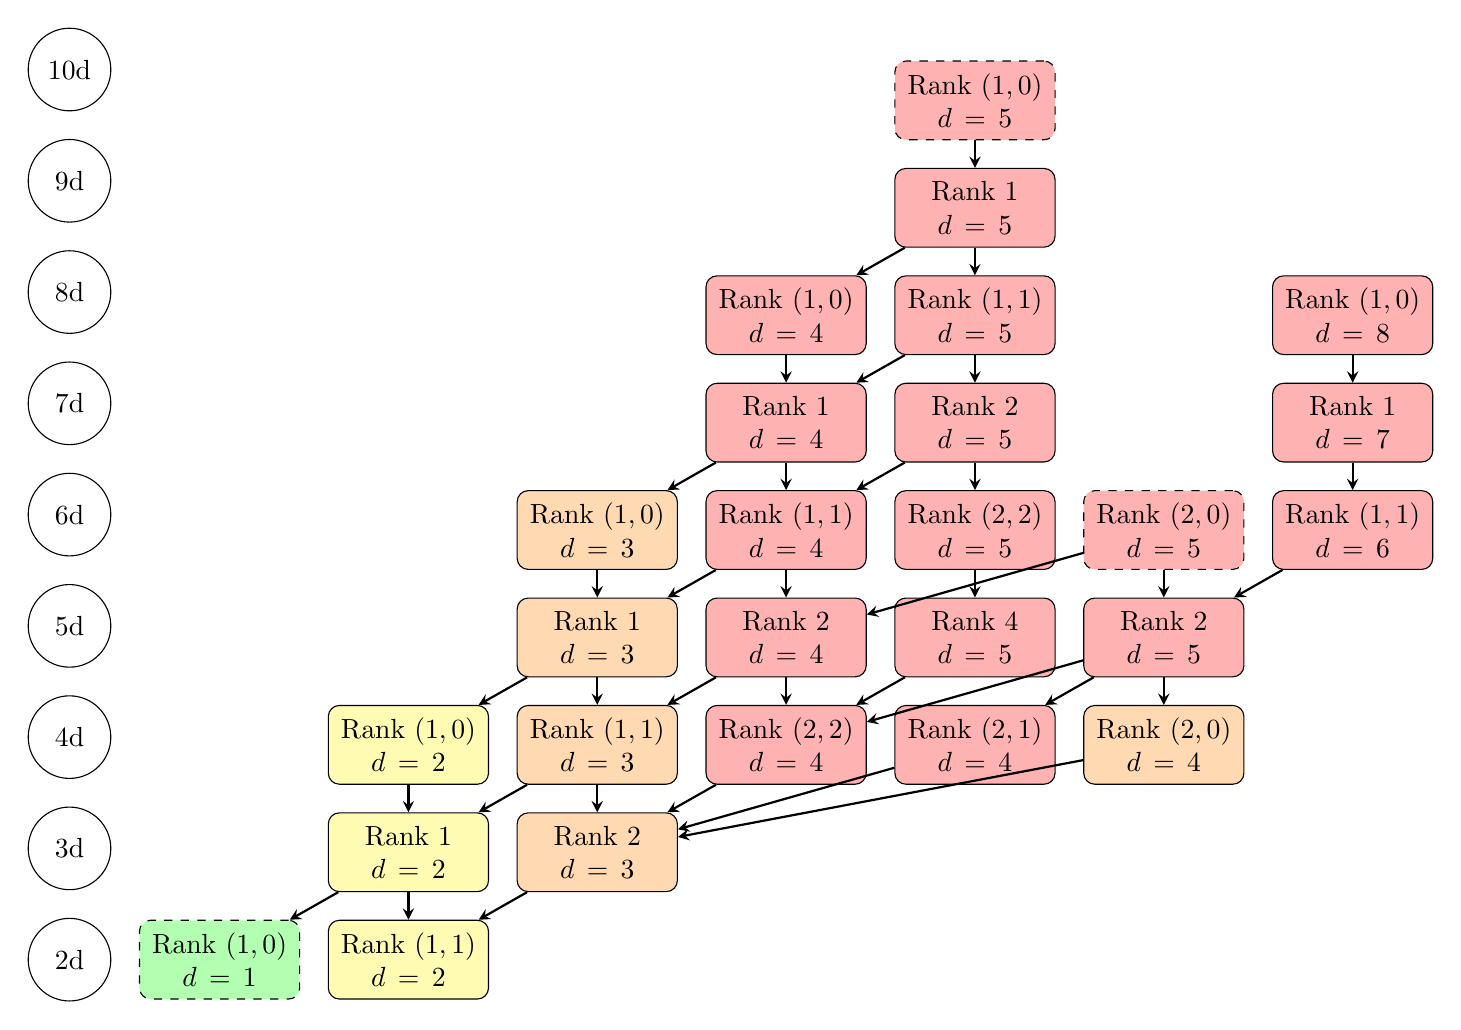
\begin{tikzpicture}[node distance=0.35cm and 0.35cm, text width=1.8cm]
\node (101) [s16chiral] {Rank $(1, 0)$ $d=5$};
\node (91) [s16, below=of 101] {Rank $1$ $d=5$};
\node (82) [s16, below=of 91] {Rank $(1, 1)$ $d=5$};
\node (81) [s16, left=of 82] {Rank $(1, 0)$ $d=4$};
\node (825) [right=of 82] {};
\node (83) [s16, right=of 825] {Rank $(1, 0)$ $d=8$};
\node (71) [s16, below=of 81] {Rank $1$ $d=4$};
\node (72) [s16, below=of 82] {Rank $2$ $d=5$};
\node (73) [s16, below=of 83] {Rank $1$ $d=7$};
\node (62) [s16, below=of 71] {Rank $(1, 1)$ $d=4$};
\node (61) [s8, left=of 62] {Rank $(1, 0)$ $d=3$};
\node (63) [s16, below=of 72] {Rank $(2, 2)$ $d=5$};
\node (64) [s16chiral, right=of 63] {Rank $(2, 0)$ $d=5$};
\node (65) [s16, below=of 73, right=of 64] {Rank $(1, 1)$ $d=6$};
\node (51) [s8, below=of 61] {Rank $1$ $d=3$};
\node (52) [s16, below=of 62] {Rank $2$ $d=4$};
\node (53) [s16, below=of 63] {Rank $4$ $d=5$};
\node (54) [s16, below=of 64] {Rank $2$ $d=5$};
\node (42) [s8, below=of 51] {Rank $(1, 1)$ $d=3$};
\node (41) [s4, left=of 42] {Rank $(1, 0)$ $d=2$};
\node (43) [s16, right=of 42] {Rank $(2, 2)$ $d=4$};
\node (44) [s16, right=of 43] {Rank $(2, 1)$ $d=4$};
\node (45) [s8, right=of 44] {Rank $(2, 0)$ $d=4$};
\node (31) [s4, below=of 41] {Rank $1$ $d=2$};
\node (32) [s8, below=of 42] {Rank $2$ $d=3$};
\node (22) [s4, below=of 31] {Rank $(1, 1)$ $d=2$};
\node (21) [s2chiral, left=of 22] {Rank $(1, 0)$ $d=1$};

\draw[arrow] (101) -- (91);
\draw[arrow] (91) -- (81);
\draw[arrow] (91) -- (82);
\draw[arrow] (81) -- (71);
\draw[arrow] (82) -- (71);
\draw[arrow] (82) -- (72);
\draw[arrow] (83) -- (73);
\draw[arrow] (71) -- (61);
\draw[arrow] (71) -- (62);
\draw[arrow] (72) -- (62);
\draw[arrow] (72) -- (63);
\draw[arrow] (73) -- (65);
\draw[arrow] (61) -- (51);
\draw[arrow] (62) -- (51);
\draw[arrow] (62) -- (52);
\draw[arrow] (63) -- (53);
\draw[arrow] (64) -- (52);
\draw[arrow] (64) -- (54);
\draw[arrow] (65) -- (54);
\draw[arrow] (51) -- (41);
\draw[arrow] (51) -- (42);
\draw[arrow] (52) -- (42);
\draw[arrow] (52) -- (43);
\draw[arrow] (53) -- (43);
\draw[arrow] (54) -- (43);
\draw[arrow] (54) -- (44);
\draw[arrow] (54) -- (45);
\draw[arrow] (41) -- (31);
\draw[arrow] (42) -- (31);
\draw[arrow] (42) -- (32);
\draw[arrow] (43) -- (32);
\draw[arrow] (44) -- (32);
\draw[arrow] (45) -- (32);
\draw[arrow] (31) -- (21);
\draw[arrow] (31) -- (22);
\draw[arrow] (32) -- (22);

\node (2d) [dimension, left=of 21] {2d};
\node (3d) [dimension, above=of 2d] {3d};
\node (4d) [dimension, above=of 3d] {4d};
\node (5d) [dimension, above=of 4d] {5d};
\node (6d) [dimension, above=of 5d] {6d};
\node (7d) [dimension, above=of 6d] {7d};
\node (8d) [dimension, above=of 7d] {8d};
\node (9d) [dimension, above=of 8d] {9d};
\node (10d) [dimension, above=of 9d] {10d};
\end{tikzpicture}
\caption{Orbits of square-zero supercharges.}
\label{fig:superchargeorbits}
\end{figure}
%\end{landscape}

\subsection{Standard Equivalences Between Classical Field Theories}
In this section, we will collect some standard lemmas that we'll use to simplify the descriptions of twisted supersymmetric field theories below.

\begin{lemma} \label{symplectomorphism_lemma}
A linear symplectomorphism $F \colon \mc E^\bullet \to \mc E^\bullet$ induces an equivalence of theories between $(\mc E^\bullet, Q, \omega, I)$ and $(\mc E^\bullet, F^*Q, \omega, F^*I)$.
\end{lemma}

\brian{I may be optimistic, but shouldn't the lemmas below all follow from the fact that the category we are working with is a Grothendieck abelian category? In any case, I do like that we've stated them clearly.} \chris{I'm not sure what you have in mind (for instance I'm not sure why you would need the Grothendieck condition there), but I think the lemmas below should be formally immediate in this dg category of differentiable cochain complexes setting (like the first one follows in any context where you have an exact sequence $0 \to A \to B \to C \to 0$ and the fact that if $C$ is equivalent to 0 then $A \to B$ is an equivalence, or the same with $A$ and $B \to C$.)}

\begin{lemma} \label{inclusion_and_projection_lemma}
Let $(\mc E^\bullet, Q)$ be a cochain complex, and let $(\mc C^\bullet, Q')$ be a contractible cochain complex.
\begin{enumerate}
 \item Let $F \colon \mc C^\bullet \to \mc E^\bullet$ be a degree 1 map making $(\mc C^\bullet \overset F\to \mc E^\bullet)$ into a cochain complex.  Then the canonical inclusion $\mc E^\bullet \to (\mc C^\bullet \overset F\to \mc E^\bullet)$ is a quasi-isomorphism.
 \item Let $F' \colon \mc E^\bullet \to \mc C^\bullet$ be a degree 1 map making $(\mc E^\bullet \overset {F'}\to \mc C^\bullet)$ into a cochain complex.  Then the canonical projection $(\mc E^\bullet \overset {F'}\to \mc C^\bullet) \to \mc E^\bullet$ is a quasi-isomorphism.
\end{enumerate}
\end{lemma}

\begin{lemma} \label{symplectic_composite_lemma}
Let $(\mc E^\bullet,Q)$ be a cochain complex, let $(\mc C_1^\bullet, Q_1)$ and $(\mc C_2^\bullet, Q_2)$ be contractible cochain complexes, and let $\mc C_1^\bullet \overset{F_1}\to \mc E^\bullet \overset{F_2}\to \mc C_2^\bullet$ be a pair of degree 1 maps so that the differential $Q + Q_1 + Q_2 + F_1 + F_2$ on the total complex squares to 0.  Suppose the graded vector space $\mc E^\bullet \oplus \mc C_1^\bullet \oplus C_2^\bullet$ is equipped with a $-1$-shifted symplectic structure so that $\mc C_1^\bullet \oplus \mc C_2^\bullet$ is a symplectic subspace.  Then the cochain map 
\begin{equation}
\label{symp_composite_eqn}\mc E^\bullet \to (\mc C_1^\bullet \overset{F_1}\to \mc E^\bullet \overset{F_2}\to \mc C_2^\bullet)
\end{equation}
obtained as the composite of the projection from Lemma \ref{inclusion_and_projection_lemma} (2) with a quasi-inverse to the inclusion from Lemma \ref{inclusion_and_projection_lemma} (1) is a symplectomorphism.
\end{lemma}

\begin{lemma} \label{interaction_pullback_lemma}
In the set-up of Lemma \ref{symplectic_composite_lemma}, suppose we're given an interaction $I$ on the graded vector space $\mc E^\bullet \oplus \mc C_1^\bullet \oplus \mc C_2^\bullet$, which pulls back to $I'$ under the inclusion of $\mc E^\bullet$.  Suppose that all monomial summands of the interaction $I$ which depend on fields in $\mc C_2^\bullet$ also depend on fields in $\mc C_1^\bullet$. Then the map \ref{symp_composite_eqn} is compatible with the interactions $I$ and $I'$
\end{lemma}

\begin{proof}
We defined a quasi-isomorphism of cochain complexes in Lemma \ref{symplectic_composite_lemma} to be the composite $F$ of the inclusion $i$ of $\mc E^\bullet \oplus \mc C_2^\bullet$ with a quasi-inverse to the projection onto $\mc E^\bullet$: this composite map is a twisted inclusion $\mc E^\bullet \to \mc E^\bullet \oplus \mc C_1^\bullet \oplus \mc C_2^\bullet$ of the form $F \colon \phi \mapsto (\phi, 0, f(\phi))$ for some linear map $f$.  Because, by the hypothesis, all monomial summands of $I$ involving fields in $\mc C_2^\bullet$ also include fields in $\mc C_1^\bullet$, the pullback of $I$ under the map $F$ coincides with the pullback of $I$ under the inclusion map $\phi \mapsto (\phi, 0, 0)$ as required.
\end{proof}


\subsection{Dimension 10}
We'll begin our discussing of twists of super Yang-Mills theory by studying the twist of 10-dimensional $\mc N=(1,0)$ super Yang-Mills theory, with the supersymmetry action we analyzed in Section \ref{SUSY_action_section}.  In the 10d $\mc N=(1,0)$ supersymmetry algebra there is a unique $\Spin(10)$ orbit of non-trivial square-zero supercharges given by the locus of pure spinors.  These square-zero supercharges are holomorphic.

Fix a non-trivial pure spinor $Q$, or equivalently, fix a Calabi-Yau structure on $\RR^{10}$.  The stabilizer of $Q$ in $\Spin(10)$ is isomorphic to $\SU(5)$.  Let us first, therefore, decompose the component fields of 10d super Yang-Mills theory into sections of the associated bundles to irreducible representations of $\SU(5)$.  The BRST fields split as follows:
\begin{align*}
c &\mapsto c \in \Omega^0(\CC^5; \gg) \\
A &\mapsto A_{0, 1} + A_{1, 0} \in \Omega^{0,1}(\CC^5; \gg) \oplus \Omega^{1,0}(\CC^5; \gg)\\
\lambda &\mapsto \chi + \psi + B \in \Omega^0(\CC^5; \gg) \oplus \Omega^{1,0}(\CC^5; \gg) \oplus \Omega^{0,2}(\CC^5; \gg). 
\end{align*}

In terms of these component fields, the BV action functional can be written in the following way.  We'll split the action functional up into the BRST action and the antifield action.
\begin{align*}
S_{\mr{BRST}} &= \int \d^5z \left(\Lambda^2 \langle F_{0,2} \wedge F_{2,0}\rangle + \frac 12 |\Lambda F_{1,1}|^2 + \Lambda( \chi \wedge (\ol \dd_{A_{0,1}} \psi))  + \Lambda^2(B \wedge (\dd_{A_{1,0}} \psi))\right) \Omega + (B \wedge \ol \dd_{A_{0,1}} B) \\
S_{\mr{anti}} &= \int \d^5z \langle \dd_{A_{1,0}}c, A_{1,0}^\vee \rangle +  \langle \ol \dd_{A_{0,1}}c, A_{0,1}^\vee \rangle + \langle [c,c], c^\vee \rangle + \langle [\chi,c], \chi^\vee \rangle + \langle [\psi,c], \psi^\vee \rangle + \langle [B,c], B^\vee \rangle,
\end{align*}
where $F_{i,j}$ is the $(i,j)$-form component of the curvature of the gauge field $A_{0, 1} + A_{1, 0}$, and $\Omega$ is the Calabi-Yau $(0,5)$-form.  Similarly, we can write explicitly the $L_\infty$ interaction functional associated to the action of the square 0 supercharge $Q$.  It has a quadratic and a cubic component given by
\begin{align*}
I^{(1)} &= \int \langle A_{1,0}^\vee, \psi \rangle + \langle \chi^\vee \Lambda F_{1,1} \rangle + \langle B^\vee, F_{0,2} \rangle \\
I^{(2)} &= \frac 12 \int \d^5z \Omega |\chi^\vee|^2.
\end{align*}
The twisted action functional is obtained by adding these terms to the original BV action functional.

We can now calculate the 10d holomorphic twist.  This calculation is originally due to Baulieu \cite{Baulieu}.

\begin{theorem}\label{10d_twist_thm}
The holomorphic twist of 10d super Yang-Mills theory on a Calabi-Yau 5-fold $X_5$ is equivalent to holomorphic Chern-Simons theory on $X_5$.
\end{theorem}

\begin{remark}
From the point of view of supersymmetry, the twisted theory is only $\ZZ/2\ZZ$-graded, because the R-symmetry group is trivial, so there is no possible R-charge with which to regrade the twisted theory to make it $\ZZ$-graded.  
This is of course compatible with our conventions for holomorphic Chern-Simons: holomorphic Chern-Simons (with values in an ordinary Lie algebra) on an odd dimensional Calabi-Yau only defines a $\ZZ/2$-graded theory (unless $d=3$, where this can be lifted to a $\ZZ$-grading). 
As a consequence, the twisted BV-BRST complex only has an odd symplectic pairing, not a $(-1)$-symplectic pairing.
\end{remark}

\begin{proof}
We'll prove this equivalence by first describing an equivalence of the underlying classical theories, as the composite of several maps, then showing that this equivalence is compatible with the two interaction functionals, and therefore defines a morphism of classical field theories, and finally observing that by Lemma \ref{free_int_ss_lemma} this morphism is automatically an equivalence.

\begin{enumerate}
 \item The first part of our equivalence of classical field theories will be a simple change of variables.  Let $\chi'^\vee = \chi^\vee + \Lambda F_{1,1}$, and dually let $\chi' = \chi + \Lambda F_{1,1}^\vee$.  In terms of $\chi'$, the quadratic part of the twisted action functional becomes
 \begin{align*}
  S^Q &= \int \d^5z \left(\Lambda^2 \langle \ol \dd A_{0,1} \wedge \dd A_{1,0} \rangle + \frac 12 |\chi'^\vee|^2 + \Lambda( \chi' \wedge (\ol \dd \psi)) - \Lambda^2(\dd A_{0,1} \wedge \ol \dd \psi) + \Lambda^2(B \wedge (\dd \psi))\right) \Omega + (B \wedge \ol \dd B) \\
  &\quad + \langle \dd c, A_{1,0}^\vee \rangle +  \langle \ol \dd c, A_{0,1}^\vee \rangle + \langle A_{1,0}^\vee, \psi \rangle + \langle B^\vee, \ol \dd A_{0,1} \rangle.
 \end{align*}
 The classical BV complex associated to the theory after performing this change of variables is quasi-isomorphic to the classical BV complex of the original theory according to Lemma \ref{symplectomorphism_lemma}.  However, after performing the change of variables, the classical BV complex takes the form $(\Omega^0(\CC^5; \gg)_{\chi'^\vee} \overset \id \to \Pi\Omega^0(\CC^5; \gg)_{\chi'}) \to \mc E^\bullet$, where $\mc E^\bullet$ is the part of the BV complex generated by all fields other than $\chi'$ and $\chi'^\vee$, and where the map into $\mc E^\bullet$ is given by the map $\ol \dd$ from $\chi$ to $\psi^\vee$.  Therefore the inclusion of the complex $\mc E^\bullet$ is a quasi-isomorphism by Lemma \ref{inclusion_and_projection_lemma}.  We think of this as ``integrating out'' the field $\chi'$ and its antifield.
 
 \item We'll now use a similar trick to integrate out the fields $\psi, A_{1,0}$ and their antifields.  We've argued in step 1 that the free part of the $Q$-twisted theory is equivalent to the theory with action functional 
 \[  S^Q = \int \d^5z \left(\Lambda^2 \langle \ol \dd A_{0,1} \wedge \dd A_{1,0} \rangle + \Lambda^2(B \wedge (\dd \psi))\right) \Omega + (B \wedge \ol \dd B) + \langle \dd c, A_{1,0}^\vee \rangle +  \langle \ol \dd c, A_{0,1}^\vee \rangle + \langle A_{1,0}^\vee, \psi \rangle + \langle B^\vee, \ol \dd A_{0,1} \rangle.\]
 We'll begin, as in step 1, by performing a linear change of variables, setting $A'_{1,0} = A_{1,0} - \ol{A_{0,1}}$, and performing the dual change of variables on the antifields.  This change of variables has the effect of eliminating the term $\langle \dd c, A_{1,0}^\vee \rangle$ from the quadratic part of the action. \chris{This isn't quite right I think.  We need to kill that term, however, for the below argument to work.  Can we fix it?}
 
 Observe that the classical BV complex associated to this action functional can now be written in the following form:
 \[\xymatrix{
 &&\Omega^{1,0}(\CC^5;\gg)_\psi \ar[dl] \ar[dr] \ar[r] &\Omega^{1,0}(\CC^5;\gg)_{{A'}_{1,0}} \ar[dr]\\
 \Omega^0(\CC^5;\gg)_c \ar[r] &\Omega^{0,1}(\CC^5;\gg)_{A_{0,1}}  \ar[dl] \ar[r] &\Omega^{0,2}(\CC^5;\gg)_{B} \ar[dl]\ar[r] &\Omega^{0,3}(\CC^5;\gg)_{B^\vee} \ar[r] &\Omega^{0,4}(\CC^5;\gg)_{A_{0,1}^\vee} \ar[dlll] \ar[r] &\Omega^{0,5}(\CC^5;\gg)_{c^\vee} \\
 \Omega^{4,0}(\CC^5;\gg)_{{A'}_{1,0}^\vee} \ar[r]   &\Omega^{4,0}(\CC^5;\gg)_{\psi^\vee},
 }\]
 where the first and third rows are dual under the symplectic pairing.  This is exactly in the form required to apply Lemma \ref{symplectic_composite_lemma}, so applying that result tells us that the underlying free theory of the twisted 10d super Yang Mills theory is equivalent to the middle row alone, i.e. the Dolbeault complex, which is exactly the free part of holomorphic Chern-Simons theory on $\CC^5$.
 
 \item Now, let's understand how the interaction functional behaves under this equivalence of classical field theories.  The morphism from step 1 is just given by an inclusion, so the interaction on twisted 10d Yang-Mills theory is compatible with the interaction evaluated at $\chi'=\chi'^\vee=0$.  In order to make the same observation for the fields $\psi$ and $A_{1,0}$, we'll use Lemma \ref{interaction_pullback_lemma}, which we can apply using the observation that the antifields $A_{1,0}^\vee$ and $\psi^\vee$ only appear in the action together with the corresponding fields.  Take our original action functional after the change of variables from step 1, and set the fields $\chi, \psi, A_{1,0}$ and their antifields to zero (i.e, in the notation of Lemma \ref{interaction_pullback_lemma}, restrict the interaction to the complex $\mc E^\bullet$).  The resulting interaction is 
 \[
  I^Q = \int \d^5z (B \wedge [A_{0,1} \wedge B]) + \langle B^\vee, [A_{0,1} \wedge A_{0,1}] \rangle + \langle [c,c], c^\vee \rangle + \langle [A_{0,1}, c], A_{0,1}^\vee \rangle + \langle [B,c], B^\vee \rangle,
 \]
 which is, indeed, the interaction functional for holomorphic Chern-Simons theory.  The composite of the morphisms in steps 1 and 2 therefore defines a morphism of classical field theories from holomorphic Chern-Simons theory to twisted 10d super Yang-Mills theory.
 
 \item To conclude the proof, we only need to apply Lemma \ref{free_int_ss_lemma}.  The morphism of classical field theories that we've constructed induces an equivalence of the $E_1$ pages of the free-to-interacting spectral sequences associated to holomorphically twisted 10d super Yang-Mills theory and holomorphic Chern-Simons theory.  Because the spectral sequences are convergent, there is likewise an equivalence of the $E_\infty$ pages, i.e. an equivalence of classical field theories.
\end{enumerate}
\end{proof}

The above argument can be applied identically on a general Calabi-Yau 5-fold $X$.
\brian{How do we place 10d YM on an arbitrary 5-fold? 
Are you using something about sugra?
} \chris{Not an arbitrary 5-fold, but just Calabi-Yau.  I'm not thinking of using sugra.  Instead I want to say that a Calabi-Yau 5-fold has a principal $\SU(5)$ frame bundle.  Take the fields to be sections of the associated vector bundles under the appropriate representations, then use the same action functional: the Lagrangian density is $\SU(5)$ invariant and so will define a density on the 5-fold.}


\subsection{Dimension 9}
The 9-dimensional $\mc N=1$ super Yang-Mills theory is obtained by dimensional reduction of $\mc N=1$ super Yang-Mills from $\RR^{10}$ to $\RR^9$.  It has BRST fields given by a ghost, a 9d gauge field $A$, a $\gg$-valued scalar field $\phi$, and a Dirac spinor field $\lambda$.

\chris{There is a single non-zero class of square zero supercharges in 9d, which are minimal (i.e. have 5d image).  They are stabilized by $\SU(4)$.  The twisted theory is only $\ZZ/2\ZZ$-graded.}

\begin{theorem}
The minimal twist of 9d super Yang-Mills theory on the product of a Calabi-Yau 4-fold $X_4$ and an oriented 1-manifold $L = \RR$ or $S^1$ is equivalent to mixed Chern-Simons theory on $X_4 \times L_\mr{dR}$.
\end{theorem}

The relevant fields for this calculation are those component fields which survived the 10d holomorphic twist of Theorem \ref{10d_twist_thm}.  These fields, in the BRST formalism, decompose as
\begin{align*}
B^{10} &= B + A \wedge \d \ol z^5 \in (\Omega^{0,2}(\CC^4; \gg) \oplus \Omega^{0,1}(\CC^4; \gg)) \otimes \Omega^0(\RR x_9) \\
A^{10}_{0,1} &= A' + \phi \d \ol z^5 \in (\Omega^{0,1}(\CC^4; \gg) \oplus \Omega^0(\CC^4; \gg)) \otimes \Omega^0(\RR x_9)
\end{align*}
along with the ghost $c$. \chris{can prove the theorem by the same argument as in 10d, or using dimensional reduction.}

\subsection{Dimension 8}

% \cN=1 SYM, three twists

\subsection{Dimension 7}

% \cN=1 SYM, three twists identical to dimension 8

\subsection{Dimension 6}

% \cN=(1, 1) SYM, three twists identical to dimension 8

% \cN=(1, 0) SYM with matter in a pseudo-real representation, one twist. 

\subsection{Dimension 5}

% \cN=2 SYM, three twists
% \cN=1 SYM with matter in a pseudo-real representation, one twist.

\subsection{Dimension 4}

% \cN=4 SYM
% \cN=2 SYM with matter in a pseudo-real representation
% \cN=1 SYM with matter in a complex representation

\subsubsection{$\cN=1$ SYM with matter} 

Let $R$ be a complex representation of $\mf g$.

The matter sector of the theory is labeled by the BRST fields:
\begin{itemize}
\item Two scalars $\varphi_{\pm} \in C^\infty (\RR^4) \otimes R$;
\item Weyl fermions $\psi_{\pm} \in \Pi C^\infty(\RR^4) \otimes S_{\pm} \otimes R$ 
\end{itemize} 
which together define the (abelian) local Lie algebra
\[
\mathcal E_{\rm matter}^{\cN=1} = C^\infty (\RR^4) \otimes R^{\oplus 2} \oplus  \Pi C^\infty(\RR^4) \otimes (S_{+}  \otimes R \oplus S_- \otimes R) .
\]
\subsection{Dimension 3}

% \cN=8 SYM
% \cN=4 SYM with matter in a pseudo-real representation
% \cN=2 SYM with matter in a complex representation

\subsection{Dimension 2}

% \cN=(8, 8) SYM
% \cN=(4, 4) SYM with matter in a pseudo-real representation
% \cN=(2, 2) SYM with matter in a complex representation
%BRIAN FIND REFERENCE OF BELOW
% \cN=(0,2) SYM with matter 
% \cN=(0,4) SYM with matter
% \cN=(0,8) SYM with matter


\appendix

\section{Functional analysis} \label{appx: top}

\def\CVS{{\rm CVS}}
\def\DVS{{\rm DVS}}

\brian{We can put all our conventions for topological vector spaces, largely borrowed from \cite{CG1}, here. }

\subsection{Notations and conventions}

\begin{dfn}
Let $M$ be a manifold and $E$ a (graded) vector bundle on $M$.  
For any open set $U \subset M$, define the following notations:
\begin{itemize}
\item $\cE(U)$ denotes the graded vector space of smooth sections supported on $U$;
\item $\cE_c(U)$ denotes the graded vector space of compactly supported smooth sections on $U$;
\item $\Bar{\cE}(U)$ denotes the graded vector space of distributional smooth sections on $U$;
\item $\Bar{\cE}_c(U)$ denotes the graded vector space of compactly supported distributional smooth sections on $U$.
\end{itemize}
\end{dfn}

If $E$ is a vector bundle, let $E^!$ denote the ``Verdier dual" vector bundle defined by $E^* \otimes {\rm Dens}_M$, where $E^*$ is the usual linear dual vector bundle. 
For an open set $U \subset M$ let 
\[
\cE(U)^\vee = \Bar{\cE}^!_c(U)
\]
be the continuous, or distributional, dual to $\cE(U)$. 

\brian{recall definition of CVS. all our familiar spaces above are in $\CVS$. talk about tensor products.}

\begin{prop}
Let $E,F$ be vector bundles on $M,N$ respectively.
Then
\[
\cE(M) \Hat{\otimes}_\beta \cF(N) \cong \Gamma(M \times N, E \boxtimes F)
\]
\end{prop}

\begin{dfn}\label{dfn: fnl}
Let $E$ be a vector bundle on $M$ and $U \subset M$.
The {\bf completed algebra of functions} on $\cE(U)$ is
\[
\cO(\cE(U)) = \prod_{n = 0}^\infty {\rm Hom}_{\rm CVS} \left(\cE(U)^{\Hat{\otimes}_\beta n}, \CC\right)_{S_n} .
\]
On global sections, we use the notation $\cO(\cE) = \cO(\cE(M))$. 
\end{dfn}

\subsection{Differentiable vector spaces}
\def\Mfld{{\rm Mfld}}

Let $\Mfld$ denote the site of smooth manifolds (of arbitrary dimension) where the morphisms are smooth maps, and a cover $f : X \to Y$ is a surjective local diffeomorphism.  

\begin{dfn} 
We use the following notations and naming conventions for sheaves on $\Mfld$:
\begin{itemize}
\item a {\bf smooth vector space} is a sheaf of vector spaces on $\Mfld$.
\item Let $C^\infty$ denote the smooth vector space which assigns the space of smooth functions $C^\infty(X)$ to a smooth manifold $X$.
\item a $C^\infty$-{\bf module} is a smooth vector space $V$ equipped with a structure of a module over $C^\infty$. 
If $V$ is a $C^\infty$-module, we denote $C^\infty(X, V) := V(X)$, the valued of $V$ on the smooth manifold $X$.
\item a {\bf differentiable vector space} is a $C^\infty$-module $V$ equipped with a flat connection
\[
\nabla_{X,V} : C^\infty(X, V) \to \Omega^1(X, V)
\]
for every smooth manifold $X$, which is required to be natural under pullbacks:
\[
f^* \circ \nabla_{Y,V} = \nabla_{X,V} \circ f^*
\]
for every smooth map $f : X \to Y$. 
A map of differentiable vector spaces is a map of $C^\infty$-modules which intertwines the flat connections. 
\end{itemize}
\end{dfn}

\subsection{Homological algebra}

There is a functor
\[
dif_c : \CVS \to \DVS 
\]
from the category of convenient vector spaces to the category of differentiable vector spaces. 
This functor does not preserve cokernels, so $dif_c$ does not preserve cohomology. 
In particular, with a naive definition of quasi-isomorphism internal to $\CVS$, the functor $dif_c$ does not preserve quasi-isomorphisms. 
To avoid this issue, we make the following definition. 

\begin{dfn}
Suppose $V,W$ are cochain complexes in convenient vector spaces. 
A cochain map $f : V \to W$ is a {\bf quasi-isomorphism} if the map
\[
dif_c (f) : dif_c(V) \to dif_c(W)
\]
is a quasi-isomorphism of differentiable vector spaces.
\end{dfn}

The cochain complexes arising in classical field theory are naturally convenient vector spaces. 
The above definition is used in what we mean by quasi-isomorphism between classical field theories, as in Definition \brian{??}.

Throughout the paper we make use of familiar manipulations with spectral sequences arising from filtrations of cochain complexes internal to differentiable vector spaces. 
A main tool is the classical Eilenberg-Moore comparison theorem, which is stated as follows.

\begin{thm}[Eilenberg-Moore Comparison]
Let $f : V \to W$ be a map of filtered cochain complexes in an AB4 abelian category.
Suppose, for each integer $n$ there exists an integer $p$ such that $F_p V^n = 0 = F_p W^n$.
If there is an integer $r \geq 0$ such that the induced map on the $r$th page of the corresponding spectral sequences 
\[
f_r^{pq} :  E_r^{pq} V \to E_r^{pq} W
\]
is an isomorphism for all $p,q$, then $f : V \to W$ is a quasi-isomorphism. 
\end{thm}

The following is the natural definition of a filtered differentiable cochain complex. 

\begin{dfn}
A {\bf filtered differentiable cochain complex} is a sequence of differentiable cochain complexes
\[
\cdots \to F_{n-1} V \to F_{n} V \to F_{n+1}V \to \cdots
\]
where each map is a monomorphism in each cohomological degree. 
A filtered differentiable cochain complex is {\bf complete} if the canonical maps $V \to V / F_n V$ induce an isomorphism $V \cong \lim V / F_n V$. 
\end{dfn}

The category of differentiable vector space is an AB4 category, in fact, it is actually a Grothendieck abelian category. 

\begin{thm}[Theorem 2.2.1 of \cite{CG1}]
The category $\DVS$ is a Grothendieck abelian category.
\end{thm}

In particular, we can freely apply the Eilenberg-Moore comparison result to the types of topological cochain complexes we come across in the BV formalism. 

\begin{dfn}\label{dfn: pro}
A {\bf differentiable pro-cochain complex} is a differentiable cochain complex $V$ with a filtration
\[
\cdots \to F_{n-1} V \to F_{n} V \to F_{n+1}V \to \cdots
\]
where each map is a monomorphism in each cohomological degree and such that the canonical maps $V \to V / F_n V$ induce a quasi-isomorphism $V \to \lim V / F_n V$. 
\end{dfn}

\subsubsection{The classical BV complex}

\begin{lem}
If $(E, \omega, Q, I)$ is the data of a classical theory on $M$, then the BV complex
\[
\left(\cO(\cE) , Q + \{I,-\}\right)
\]
is a differentiable pro-cochain complex.
More generally, the classical factorization algebra of observables $\Obs$ is a factorization algebra in differentiable pro-cochain complexes. 
\end{lem}

The above lemma used the natural filtration on the classical BV complex given by polynomial degree of observables. 
Since the free part of the differential $Q$ always preserves this filtration, the first term of the resulting spectral sequence simply computes the cohomology of the underlying free theory. 
The differential on the higher pages depend on the interacting part of of the action. 

\begin{lemma}[Free to Interacting Spectral Sequence] \label{free_int_ss_lemma}
Let $(E^\bullet, Q, \omega, I)$ be a classical field theory with polynomial interaction.  
There is a convergent spectral sequence whose $E_1$ page is the complex of classical observables of the underlying free theory, and whose $E_\infty$ page is equivalent to the complex of classical observables of the interacting theory.
\end{lemma}
\begin{proof}
The BV complex is of the form $\left(\cO(\cE), Q + \{I,-\}\right)$.
We have already exhibited \brian{this is a general fact that should go in the functional analysis section} a differentiable pro-cochain complex structure on the BV complex via the 
natural decreasing filtration 
\[
F^k \cO (\cE) = \Sym^{\geq k} (\cE^\vee)
\]
which is compatible with both $Q$ and $\{I,-\}$ separately.
The associated graded of this filtration is the differentiable cochain complex given by
\[
\left(\prod_{n \geq 0} \Sym^n (\cE^\vee) , Q \right) .
\]
This is simply the BV complex associated to the free theory based on $(E, Q, \omega)$ obtained by forgetting $I$. 
Thus, the $E_1$ page of the corresponding spectral sequence is the BV cohomology of the underlying free theory, as desired. 
\brian{shall we say a word about convergence? This must follow from completeness of the filtration in addition to boundedness in some direction of the cohomology of $\cE$.} \chris{Does convergence require that the interaction is polynomial, or alternatively does this bound the number of differentials appearing in the spectral sequence?}
\end{proof}

\begin{lemma} \label{invert_quis_lemma}
Any quasi-isomorphism of differentiable cochain complexes admits a quasi-inverse.
\end{lemma}
\brian{I think Pavel had something to say for this lemma.}

\section{$\infty$ algebra}

\brian{Not sure if this deserves a whole appendix, but it may be good to spell out what $L_\infty$ modules are, etc..}

\pagestyle{bib}
\printbibliography

\end{document}
